% 功能概述：解释最终稿中实际评测的理论到实验 Raman 域适配模型。
% 主要职责：给出覆盖掩码、来源代理、矩形多正样本损失、困难负样本及候选选择的数学定义。
% 代码库关系：由 main.tex 引入；实现对应 scripts/raman_domain_experiment.py 和 raman_top10_experiment.py。
% 图稿状态：保留 main.tex 中全流程图；作者已确认插入精简版训练机制图。
\section{Problem and Domain-Adaptation Method}\label{sec:method}
\subsection{Closed-Library Identification and Its Two Bottlenecks}
Let $\mathcal{D}=\{(y_j,m_j,c_j,s_j)\}_{j=1}^{M}$ be a library of theoretical spectra $y_j$, coverage masks $m_j$, full molecular identities $c_j$ and theoretical sources $s_j$. An experimental query $(x,m_x)$ has a target identity $c^\star$ in the library. Canonical/isomeric SMILES define exact identity, retaining stereochemistry and isotopes. A separate molecular-group key removes stereochemistry and isotopes after selecting the largest fragment; it is used for split protection and equal weighting of repeated measurements, not for exact-match scoring.

The encoder $f_\theta$ maps a spectrum and its mask to a unit vector. Similarity is $f_\theta(x,m_x)^\top f_\theta(y_j,m_j)$. We rank one fixed reference per unique structure and retain $K=10$ candidates, denoted $\mathcal{C}_{10}(x)$. Keeping a single indexed reference prevents repeated spectra of one structure from consuming several candidate slots; multiple same-identity references are nevertheless available during training.

For a selector constrained to this set, exact identification decomposes as
\begin{equation}\label{eq:ceiling}
\Pr(\hat c=c^\star)=\Pr(c^\star\in\mathcal{C}_{10})\,
\Pr(\hat c=c^\star\mid c^\star\in\mathcal{C}_{10}).
\end{equation}
The first term measures domain-adapted retrieval; the second measures disambiguation given successful retrieval. This decomposition supplies a direct diagnostic for whether failure occurs before or after language-model inference. It also prevents attributing the entire gain over unconstrained generation to LLM reasoning.

Figure~\ref{fig:domain_pipeline} connects learned retrieval, spectral evidence and constrained selection within the same inference workflow. The query $q$ and ordered candidates $C$ in the figure correspond to $x$ and $\mathcal{C}_{10}(x)$ defined above. Retrieval produces a fixed shortlist; the evidence stage supplies peak-level assignments for comparing its members. The selector returns a candidate index, preserving the retrieval ceiling in Eq.~\eqref{eq:ceiling}.



Figure~\ref{fig:domain_training} details the retrieval training mechanisms. Real experimental pairs and source-dependent synthetic views share a coverage-aware encoder; identity-based alignment and hard negatives shape the retrieval space.

\begin{figure*}[t]
\centering
% 待作者定稿后将最终图保存为 figures/raman_training_author_final.pdf，
% 再于 main.tex 导言区定义 \newcommand{\SpectraExpertFinalTrainingArtwork}{}。
% 此开关与全流程图独立；不得因草稿文件存在而自动插入。
\ifdefined\SpectraExpertFinalTrainingArtwork
  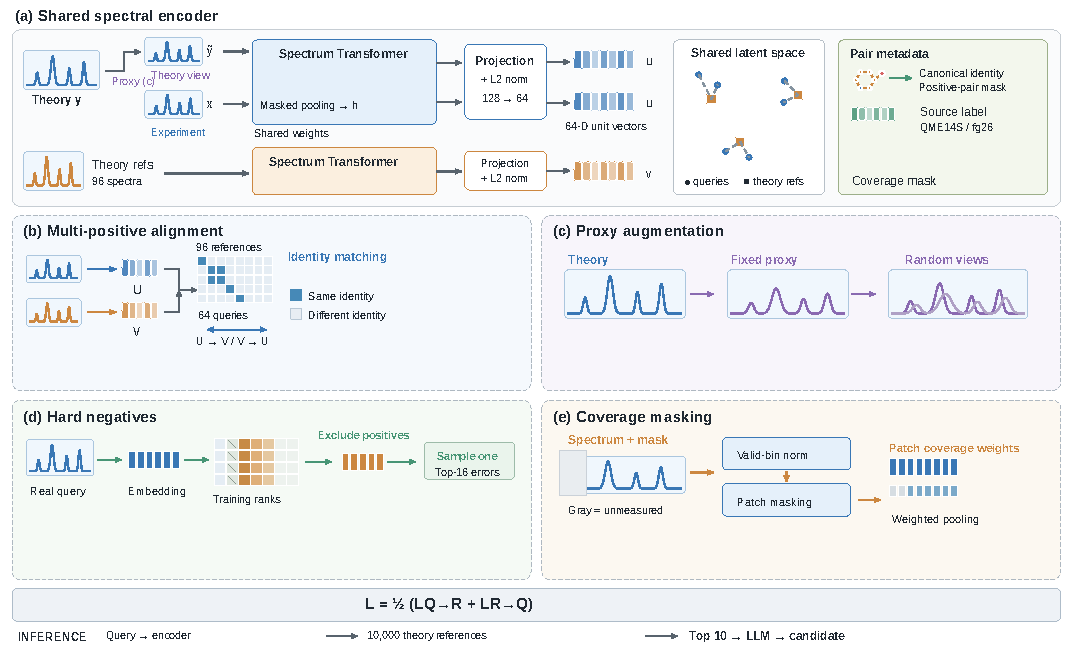
\includegraphics[width=\textwidth]{figures/raman_training_author_final.pdf}
\else
  \fbox{\begin{minipage}[c][0.50\textwidth][c]{0.96\textwidth}
    \centering\sffamily\color{gray}
    Training-method figure reserved\\[6pt]
    To be inserted after author finalization
  \end{minipage}}
\fi
\caption{Domain-adapted retrieval training. (a) A shared encoder embeds experimental queries, augmented theoretical queries and theoretical references. Blue circles and orange squares denote query and reference embeddings, respectively. (b) Contrastive learning aggregates probability over all same-identity positives. (c) Source-dependent proxies perturb frequency scale, shift and broadening. (d) Hard negatives are sampled from the top 16 incorrect training matches. (e) Coverage masks distinguish unmeasured regions from observed zeros and control normalization, attention and pooling. Proxy fitting, mining and encoder updates use training data only. All graphical examples are schematic.}
\label{fig:domain_training}
\end{figure*}

\subsection{What Is Adapted Across Domains?}\label{sec:proxy}
The transformation from a theoretical curve to a measurement can include a systematic shift in peak positions, different broadening, relative-intensity changes, baseline variation and incomplete instrument coverage. A global transformation cannot explain every molecule-specific change, but it gives an interpretable starting point for augmentation. We fit a source-dependent effective curve proxy and combine it with real spectral pairs, rather than requiring the proxy to reproduce the entire measurement process.

For source $s$, the three fitted parameters are scale $a_s$, translation $b_s$ and Gaussian width $\sigma_s$. The implementation smooths in the theoretical coordinate and then interpolates:
\begin{equation}\label{eq:proxy}
(T_{\phi_s}y)(\nu)=\frac{1}{a_s}
 (G_{\sigma_s}*y)\!\left(\frac{\nu-b_s}{a_s}\right),
\quad \phi_s=(a_s,b_s,\sigma_s).
\end{equation}
The $1/a_s$ factor preserves integrated intensity under the affine coordinate change. A Gaussian is truncated at four standard deviations; output locations are valid only when the corresponding kernel support lies within known theoretical coverage. This prevents artificial boundary values from becoming spectral evidence.

Parameters are estimated only from training pairs of the same molecular identity. For a source-specific set $\mathcal{P}_s$, let $\omega_i$ give equal total weight to each molecular group. We minimize
\begin{equation}\label{eq:proxyfit}
\phi_s^\star=\arg\min_{\phi\in\Phi}
\sum_{i\in\mathcal{P}_s}\omega_i
\bigl[1-\operatorname{cos}_{\Omega_i}(T_\phi y_i,x_i)\bigr],
\end{equation}
where $\Omega_i$ is a fixed, conservative common support valid under every bounded transformation. The fit cannot improve its score merely by moving difficult regions outside the mask. We use $a\in[0.94,1.06]$, $b\in[-40,40]$\,cm$^{-1}$ and $\sigma\in[0,12]$\,cm$^{-1}$. A coarse affine search initializes bounded derivative-free optimization. The frozen proxy used for encoder training exhausted its fitting budget and reached the broadening upper bound; these parameters are therefore an effective augmentation hypothesis, not converged estimates of instrument physics.

A single source mean underrepresents experimental variability. For each reliable training-pair affine fit, we store its joint scale/translation deviation from the source-specific median of reliable affine fits. Randomized views use no additional proxy transformation with probability 0.2, the fixed proxy with probability 0.2, and a perturbed proxy with probability 0.6. In the last case, half a sampled joint deviation is added to the source parameters and clipped to $\Phi$; the additional width is drawn uniformly between zero and the fixed width. Sampling a joint residual preserves observed scale/shift dependence without transplanting a different molecule's full residual spectrum. Reliability requires aligned correlation at least 0.25 and a correlation improvement of at least 0.05; sources with fewer than ten reliable fits use zero affine residuals.

All arms retain the same base positive-view augmentation, including small noise and contaminant peaks. Thus ``no additional proxy'' does not mean an unaugmented spectrum, and the fixed arm is not a pure physical simulator. A training experimental mask is sampled and intersected with transformed theoretical coverage. If fewer than 100 bins remain, the view falls back to its base augmentation and original coverage. No validation or test curve determines these transformations. Real experimental queries are also included directly in the loss, so deviations beyond the proxy family can affect the learned representation.

\subsection{Coverage-Aware Spectral Encoder}\label{sec:encoder}
All curves are interpolated by their physical coordinates onto 3,501 bins spanning 500--4000\,cm$^{-1}$. The associated Boolean mask distinguishes unavailable regions from measured zero intensity. For a valid-bin count $n_m=\sum_t m_t$, normalization uses only observed values:
\begin{align}
\mu_m&=n_m^{-1}\sum_t m_tx_t,\qquad
v_m=n_m^{-1}\sum_t m_t(x_t-\mu_m)^2,\\
\widetilde{x}_t&=m_t\frac{x_t-\mu_m}{\max(\sqrt{v_m},10^{-6})}.
\end{align}
Empty coverage is rejected. Without this distinction, zero padding changes the mean and variance according to measurement range, introducing a shortcut unrelated to molecular identity.

Overlapping 16-bin patches with stride 8 produce 436 tokens. A linear projection maps each patch to width 128; learned positional embeddings retain wavenumber location. Three pre-normalized Transformer layers use four attention heads, a fourfold feed-forward expansion, GELU and dropout 0.1. Entirely missing patches are excluded as attention keys and values. Let $w_p$ be the valid-bin fraction in patch $p$, and let $h_p$ be its final layer-normalized representation. We use coverage-weighted pooling and a two-layer projection:
\begin{equation}\label{eq:embedding}
\bar h=\frac{\sum_p w_ph_p}{\sum_p w_p},\qquad
z=\frac{W_2\operatorname{ReLU}(W_1\bar h)}
 {\|W_2\operatorname{ReLU}(W_1\bar h)\|_2}.
\end{equation}
Here $W_1$ maps 128 to 128 dimensions and $W_2$ maps 128 to 64; both are bias-free. Partially covered patches remain usable but contribute less to pooling. The same encoder processes experimental and theoretical spectra. Source labels determine training-view construction and sampling, but are not required as query-side encoder inputs at inference.

\subsection{Real Pairs, Multiple Positives and Hard Negatives}\label{sec:loss}
Each training step contains 32 augmented theoretical queries and 32 real experimental queries. Real pairs are sampled hierarchically by source, molecular identity and measurement, then matched to a same-identity reference from that source. This reduces domination by repeated measurements or the more common theoretical source. The reference batch contains 64 corresponding records plus 32 additional records; it is rectangular relative to the query batch.

Let $u_i$ and $v_j$ be query and reference embeddings, with identity labels $c_i$ and $d_j$. Define $P_i=\{j:c_i=d_j\}$ and $\ell_{ij}=u_i^\top v_j/\tau$, with $\tau=0.1$. The forward loss is
\begin{equation}\label{eq:contrastive}
\mathcal{L}_{Q\to R}=-\frac{1}{B_Q}\sum_i
\log\frac{\sum_{j\in P_i}\exp(\ell_{ij})}
 {\sum_{j=1}^{B_R}\exp(\ell_{ij})}.
\end{equation}
The reverse loss has the same form over references with at least one same-identity query; unsupported extra references are excluded from that reverse average. We optimize $\mathcal{L}=\tfrac12(\mathcal{L}_{Q\to R}+\mathcal{L}_{R\to Q})$. Summing the positive probability mass, rather than choosing only a diagonal match, avoids contradictory negative labels when a molecule has several theoretical records or appears repeatedly within a batch.

For the hard-negative arm, the encoder ranks training references for each training experimental query after every epoch. All references with the correct full identity are removed, and one additional reference is sampled from the 16 highest-ranked incorrect records for each of the 32 real queries. The first epoch uses random extras. Control arms also use 32 extra references, sampled randomly, so hard mining does not increase the per-step reference budget. These are model-confusable alternatives, not chemically certified negative peak assignments; the loss still determines positive membership globally by identity.

We use AdamW with learning rate $3\times10^{-4}$, weight decay $10^{-4}$ and gradient norm clipping at 1. Training runs for at most 40 epochs of 160 steps, with patience 8. Checkpoints are chosen by development group-weighted Exact@10, then Exact@1 and lower training loss. The four arms share initialization, real pairs, architecture, optimizer and reference budget. They differ in the theoretical domain view (empirical baseline, fixed proxy or random proxy) and extra-reference selection. Five-seed replication compares the empirical baseline with random proxy plus hard negatives using paired seeds 0--4.

\subsection{Spectral Evidence and a Constrained Final Decision}\label{sec:selection}
At inference, the learned similarity retrieves ten structures from the fixed theoretical index. The LLM receives an experimental peak table and candidate SMILES in retrieval order. It does not receive a target formula, target mass, true identity, candidate spectrum or similarity score. A prompt explicitly treats retrieval order as a useful prior while permitting a different choice based on peak evidence.

The optional knowledge stage matches detected peaks to frequency intervals and supplies textual vibrational assignments. The legacy knowledge base (KB) contains 181 rules and provides the matched evidence evaluated on Test-200. A separate 15-mode Raman library supports controlled development experiments. It combines source-backed frequency ranges with conservative project-defined SMARTS mappings for structural compatibility. These mappings are operational tests rather than independently validated assignments of every mode. Peaks within a 20\,cm$^{-1}$ tolerance can support a rule, but an undetected peak does not conclusively exclude a structure.

For a non-LLM control, a candidate's coverage score is the fraction of matched modes whose SMARTS are compatible with that structure. Ties retain retrieval order. A learned linear control combines inverse rank, 15 mode-compatibility indicators and coverage; it fits training-group pairwise Tanimoto differences with squared loss and $L_2$ regularization, selected on development data. Rank-only and rules-only variants isolate these feature families. These controls ask whether deterministic or fitted evidence integration explains any apparent LLM advantage.

The LLM is asked to output an index from 1 to 10, confidence and a brief explanation. Only the selected index determines the prediction. Deterministic normalization accepts an unambiguous final index or a uniquely matching candidate SMILES; conflicting or out-of-range choices remain invalid. There is no top-1 fallback, and normalization never accesses the target identity. Confidence is logged when present and does not trigger edits. The deployed policy never invents or modifies a candidate; output recovery is detailed in Section~\ref{sec:repro}.
